\documentclass{article}

\usepackage{fancyhdr}
\usepackage{amsmath}
\allowdisplaybreaks
\usepackage{amsthm}
\usepackage{amsfonts}
\usepackage{tikz}
\usepackage[plain]{algorithm}
\usepackage{algpseudocode}
\usepackage{enumitem}
\usepackage{tikz}
\usepackage{pgfplots}
\pgfplotsset{compat=1.18}
\usepgfplotslibrary{groupplots}
\usepackage{comment}

\usetikzlibrary{automata,positioning}

%
% Basic Document Settings
%

\topmargin=-0.45in
\evensidemargin=0in
\oddsidemargin=0in
\textwidth=6.5in
\textheight=9.0in
\headsep=0.25in

\linespread{1.1}

\pagestyle{fancy}
\lhead{\hmwkAuthorName}
\chead{} % empty
\rhead{\hmwkHeaderTitle}
\cfoot{\thepage}

\renewcommand\headrulewidth{0.4pt}
\renewcommand\footrulewidth{0pt}

\setlength\parindent{0pt}

%
% Homework Details
%

\newcommand{\hmwkTitle}{Homework 5}
\newcommand{\hmwkDueDate}{Monday, February 9, 2026}
\newcommand{\hmwkClass}{ICMA 216 Calculus IIIA}
\newcommand{\hmwkClassTime}{Section 1}
\newcommand{\hmwkClassInstructor}{Ruth J. Skulkhu}
\newcommand{\hmwkAuthorName}{\textbf{Jiraroj Wiruchpongsanon (6781617)}}
\newcommand{\hmwkHeaderTitle}{ICMA 216 Calculus IIIA: Homework 5}

%
% Title Page
%

\title{
    \vspace{2in}
    \textmd{\textbf{\hmwkClass:\ \hmwkTitle}}\\
    \normalsize\vspace{0.1in}\small{Due\ on\ \hmwkDueDate}\\
    \vspace{0.1in}\large{\textit{\hmwkClassInstructor\ \hmwkClassTime}}
    \vspace{3in}
}

\author{\hmwkAuthorName}
\date{}

\renewcommand{\part}[1]{\textbf{\large Part \Alph{partCounter}}\stepcounter{partCounter}\\}

%
% Helper Commands
%

\newcounter{partCounter}
\newcommand{\solution}{\textbf{\large Solution}}

\newtheorem*{theorem}{Theorem}

\theoremstyle{remark}
\newtheorem*{remark}{Remark}

\begin{document}

\maketitle
\newpage

\section*{Problem 1 (11.7 Quadric Surfaces)}
Sketch the following surfaces.
\begin{enumerate}[label=(\alph*)]
    \item $-9z^2 - 5y^2 - x + 4 = 0$
    \item $4y^2 + 9z^2 - x^2 = 0$
    \item $1 - 3z^2 - y^2 - 4x^2 = 0$
\end{enumerate}

\medskip
\solution

\begin{center}
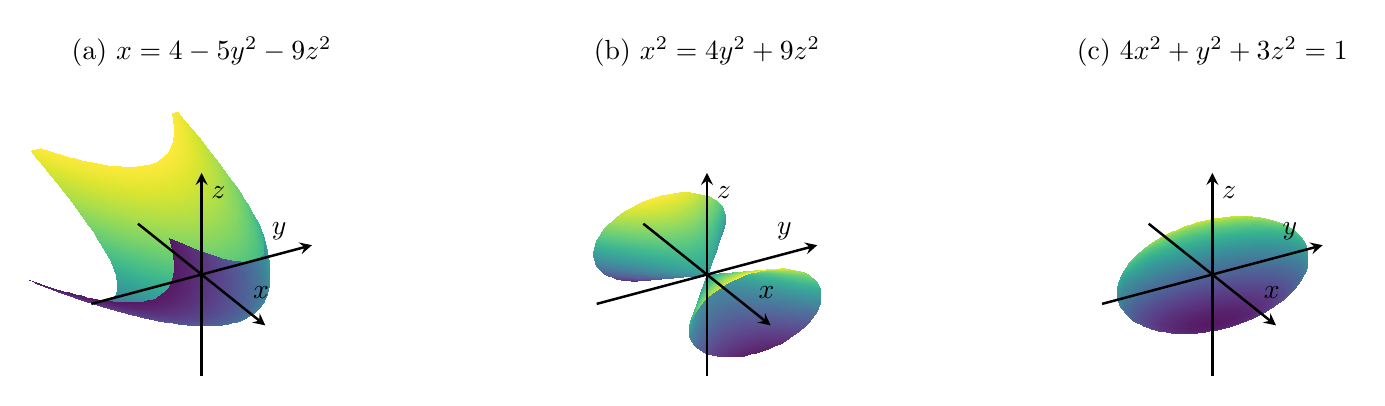
\begin{tikzpicture}
    \begin{groupplot}[
        group style={group size=3 by 1, horizontal sep=2cm},
        width=6cm, height=6.2cm,
        view={60}{30},
        axis lines=center,
        axis line style={line width=0.9pt},
        axis on top,
        ticks=none,
        xlabel={$x$}, ylabel={$y$}, zlabel={$z$},
        colormap/viridis,
    ]
        \nextgroupplot[
            title={(a)\ $x = 4 - 5y^{2} - 9z^{2}$},
            xmin=-6, xmax=6,
            ymin=-1.5, ymax=1.5,
            zmin=-1.5, zmax=1.5,
        ]
            \addplot3[
                surf, shader=interp, opacity=0.9,
                domain=-1:1,
                y domain=-1:1,
                samples=50, samples y=50
            ] ({4 - 5*x^2 - 9*y^2},{x},{y});

        \nextgroupplot[
            title={(b)\ $x^{2} = 4y^{2} + 9z^{2}$},
            xmin=-4, xmax=4,
            ymin=-2.5, ymax=2.5,
            zmin=-2.5, zmax=2.5,
        ]
            \addplot3[
                surf, shader=interp, opacity=0.88,
                domain=0:2*pi,
                y domain=-3:3,
                samples=70, samples y=36
            ] ({y},{abs(y)/2*cos(deg(x))},{abs(y)/3*sin(deg(x))});

        \nextgroupplot[
            title={(c)\ $4x^{2} + y^{2} + 3z^{2} = 1$},
            xmin=-1.2, xmax=1.2,
            ymin=-1.2, ymax=1.2,
            zmin=-1.2, zmax=1.2,
        ]
            \addplot3[
                surf, shader=interp, opacity=0.9,
                domain=0:2*pi,
                y domain=0:pi,
                samples=70, samples y=40
            ] ({0.5*sin(deg(y))*cos(deg(x))},{sin(deg(y))*sin(deg(x))},{(1/sqrt(3))*cos(deg(y))});
    \end{groupplot}
\end{tikzpicture}
\end{center}

\remark hand written plots for this problem were attached by submission.

\vspace{1em}
\hrulefill

\section*{Problem 2 (12.1 Vector Functions and Space Curves)}
Sketch the following curves.
\begin{enumerate}[label=(\alph*)]
    \item $r = (1 - t)(i + j) + t(i - j); 0 \le t \le 1$
    \item $r(t) = \langle t^4 + 1, t \rangle.$
\end{enumerate}

\medskip
\solution

\begin{center}
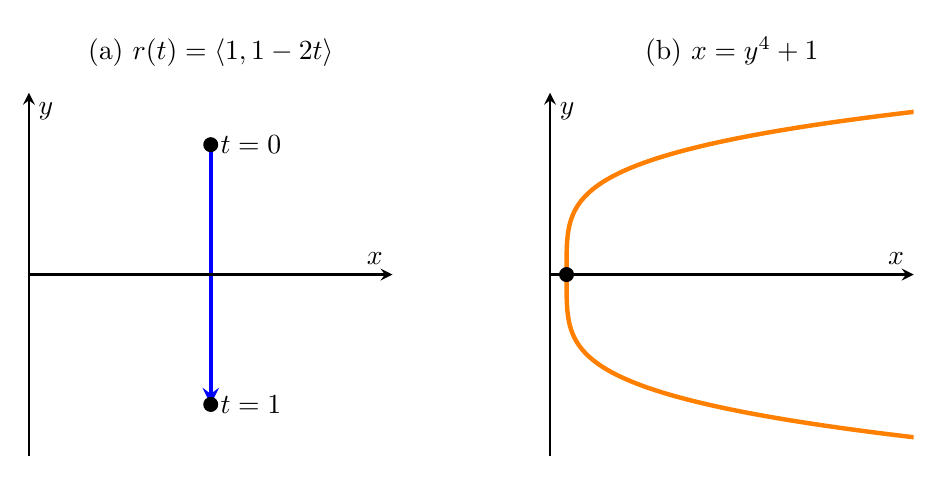
\begin{tikzpicture}
    \begin{groupplot}[
        group style={group size=2 by 1, horizontal sep=2cm},
        width=6.2cm, height=6.2cm,
        axis lines=center,
        axis line style={line width=0.9pt},
        axis on top,
        ticks=none,
        xlabel={$x$}, ylabel={$y$},
    ]
        \nextgroupplot[
            title={(a)\ $r(t) = \langle 1, 1 - 2t \rangle$},
            xmin=0.6, xmax=1.4,
            ymin=-1.4, ymax=1.4,
        ]
            \addplot[ultra thick, ->, >=stealth, color=blue]
                coordinates {(1,1) (1,-1)};
            \addplot[only marks, mark=*, mark size=2.5pt]
                coordinates {(1,1) (1,-1)};
            \node[anchor=west] at (axis cs:1,1) {$t = 0$};
            \node[anchor=west] at (axis cs:1,-1) {$t = 1$};

        \nextgroupplot[
            title={(b)\ $x = y^{4} + 1$},
            xmin=0.8, xmax=5.2,
            ymin=-1.6, ymax=1.6,
        ]
            \addplot[smooth, ultra thick, color=orange, domain=-1.5:1.5, samples=320]
                ({x^4 + 1},{x});
            \addplot[only marks, mark=*, mark size=2.5pt] coordinates {(1,0)};
    \end{groupplot}
\end{tikzpicture}
\end{center}

\vspace{1em}
\hrulefill

\newpage
\section*{Problem 3 (12.2 Calculus of Vector Functions)}
Given $r(t) = (1 + t)i + t^2 j$. Find the unit tangent vector at the point where $t = 1$.

\medskip
\solution

we could find the velocity vector by 

\[r'(t) = \frac{d}{dt}[(1 + t)i + t^{2}j] = i + 2tj\] 

at $t = 1$ gives 

\[r'(1) = i + 2j\] 

which we could calculate it's magnitude as

\[
    \lVert r'(t) \rVert = \sqrt{1^{2} + 2^{2}} = \sqrt{5}.
\]

and therefore the unit tangent vector at $t = 1$ is

\[
    \frac{r'(1)}{\lVert r'(1) \rVert} = \boxed{\frac{1}{\sqrt{5}}(i + 2j)}
\]

\vspace{1em}
\hrulefill

\section*{Problem 4 (12.2 Calculus of Vector Functions)}
Evaluate the integral
\[
    \int (e^t i + 2t j + \ln t k) \, dt.
\]

\medskip
\solution

we just integrate the vector componentwise as

\begin{itemize}
    \item{$i$-component}
    \[
    \int e^{t} \, dt = e^{t} + C_{1}$
    \]

    \item{$j$-component}
    \[
    \int 2t \, dt = t^{2} + C_{2}.
    \]

    \item{$k$-component} (integrate by parts)
    \[
    \int \ln t \, dt = t \ln t - t + C_{3}.
    \]
\end{itemize}

merge the three components, combine their constants into a single constant vector C gives
\[
    \int (e^{t} i + 2t j + \ln t k) \, dt = \boxed{e^{t} i + t^{2} j + (t \ln t - t) k + \mathbf{C}}
\]

\vspace{1em}
\hrulefill

\section*{Problem 5 (12.2 Calculus of Vector Functions)}
Find $r(t)$ if $r'(t) = t^2 i + 4t^3 j - t^2 k$ and $r(0) = k$.

\medskip
\solution

integrating $r^'(t)$ componentwise, just like the previous problem as

\[
    r(t) = \left(\int t^{2} \, dt\right) i + \left(\int 4t^{3} \, dt\right) j - \left(\int t^{2} \, dt\right) k + \mathbf{C} = \frac{t^{3}}{3} i + t^{4} j - \frac{t^{3}}{3} k + \mathbf{C},
\]

where $\mathbf{C}$ is a constant vector, then apply the initial condition $r(0) = k$
\[
    r(0) = 0i + 0j + 0k + \mathbf{C} = k.
\]

therefore, $\mathbf{C} = k$, and hence

\[
    \boxed{r(t) = \frac{t^{3}}{3} i + t^{4} j + \left(1 - \frac{t^{3}}{3}\right) k}
\]

\vspace{1em}
\hrulefill

\end{document}
